\documentclass{beamer}
\usepackage[french]{babel}
\usepackage{hyperref}
\definecolor{links}{HTML}{2A1B81}
\hypersetup{colorlinks,linkcolor=,urlcolor=links}
\usepackage{graphicx}
\usepackage{amsmath,amssymb}
\usepackage{tabularx}
\usepackage{booktabs}
\usepackage[compatibility=false]{caption}
\usepackage[toc,page]{appendix}
\usepackage{minted}
\usepackage{xspace}

\makeatletter
  \def\beamer@calltheme#1#2#3{%
    \def\beamer@themelist{#2}
    \@for\beamer@themename:=\beamer@themelist\do
    {\usepackage[{#1}]{\beamer@themelocation/#3\beamer@themename}}}

  \def\usefolder#1{
    \def\beamer@themelocation{#1}
  }
  \def\beamer@themelocation{}

\patchcmd{\minted@colorbg}{\noindent}{\medskip\noindent}{}{}
\apptocmd{\endminted@colorbg}{\par\medskip}{}{}
\makeatother

\newcolumntype{Y}{>{\centering\arraybackslash}X}

\usefolder{../theme}
\usetheme[numbering=fraction,block=fill,progressbar=frametitle]{metropolis} %Use metropolis theme

\definecolor{bg}{rgb}{0.95,0.95,0.95}
\setminted{bgcolor=bg,fontsize=\scriptsize,autogobble,mathescape,breaklines,tabsize=2}
\setmintedinline{breaklines,autogobble,fontsize=\scriptsize}
\setbeamersize{text margin left=8pt,text margin right=8pt}
\setbeamercovered{transparent}

\begin{document}

\title[C++]{Introduction à la programmation en C++}
\author[nicolas.audebert@onera.fr]{Nicolas Audebert}
\setmainfont{Fira Sans}


\AtBeginSection[]{
  \begin{frame}{Plan de la séance}
  \small \tableofcontents[currentsection]
  \end{frame}
}

\newcommand\cppi[1]{\mintinline{cpp}{#1}}
\newcommand\cpp[1]{%
  \begin{minted}{cpp}
  #1
  \end{minted}
}%

\subtitle{Préliminaires}
\date{}
\maketitle

\section{Introduction}

\begin{frame}{Avant toute chose}
  \begin{block}{Supports de cours}
    Site du cours : {\small \url{http://imagine.enpc.fr/~monasse/Info/}}\\
  	Slides : {\small \url{https://nicolas.audebert.at/teaching/}}
  \end{block}

  \begin{block}{Organisation}
    \begin{itemize}
        \item 12 séances
	\item Cours magistral de 8h30 à 9h30 puis TP de 9h45 à 11h15
        \item TPs à rendre chaque semaine sur \href{https://educnet.enpc.fr}{\textbf{Educnet}}
    \end{itemize}
  \end{block}

\end{frame}


\section{L'ordinateur et les langages}

\begin{frame}{Composants de l'ordinateur}
	\centering
	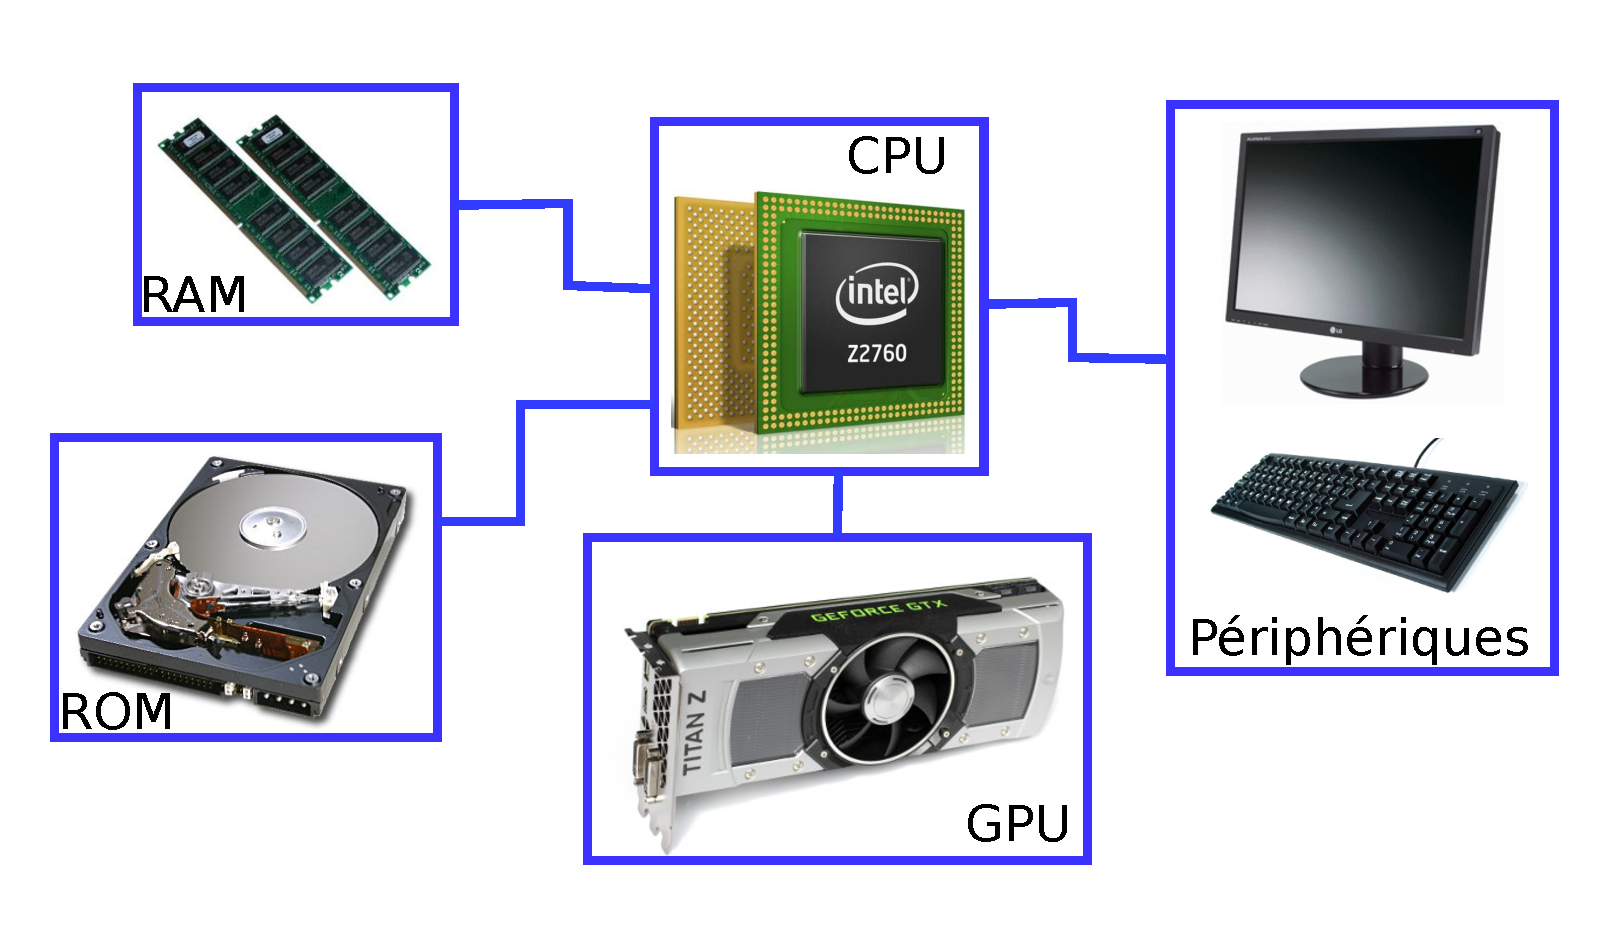
\includegraphics[width=\linewidth]{images/ordi_5.pdf}
	%\only<1>{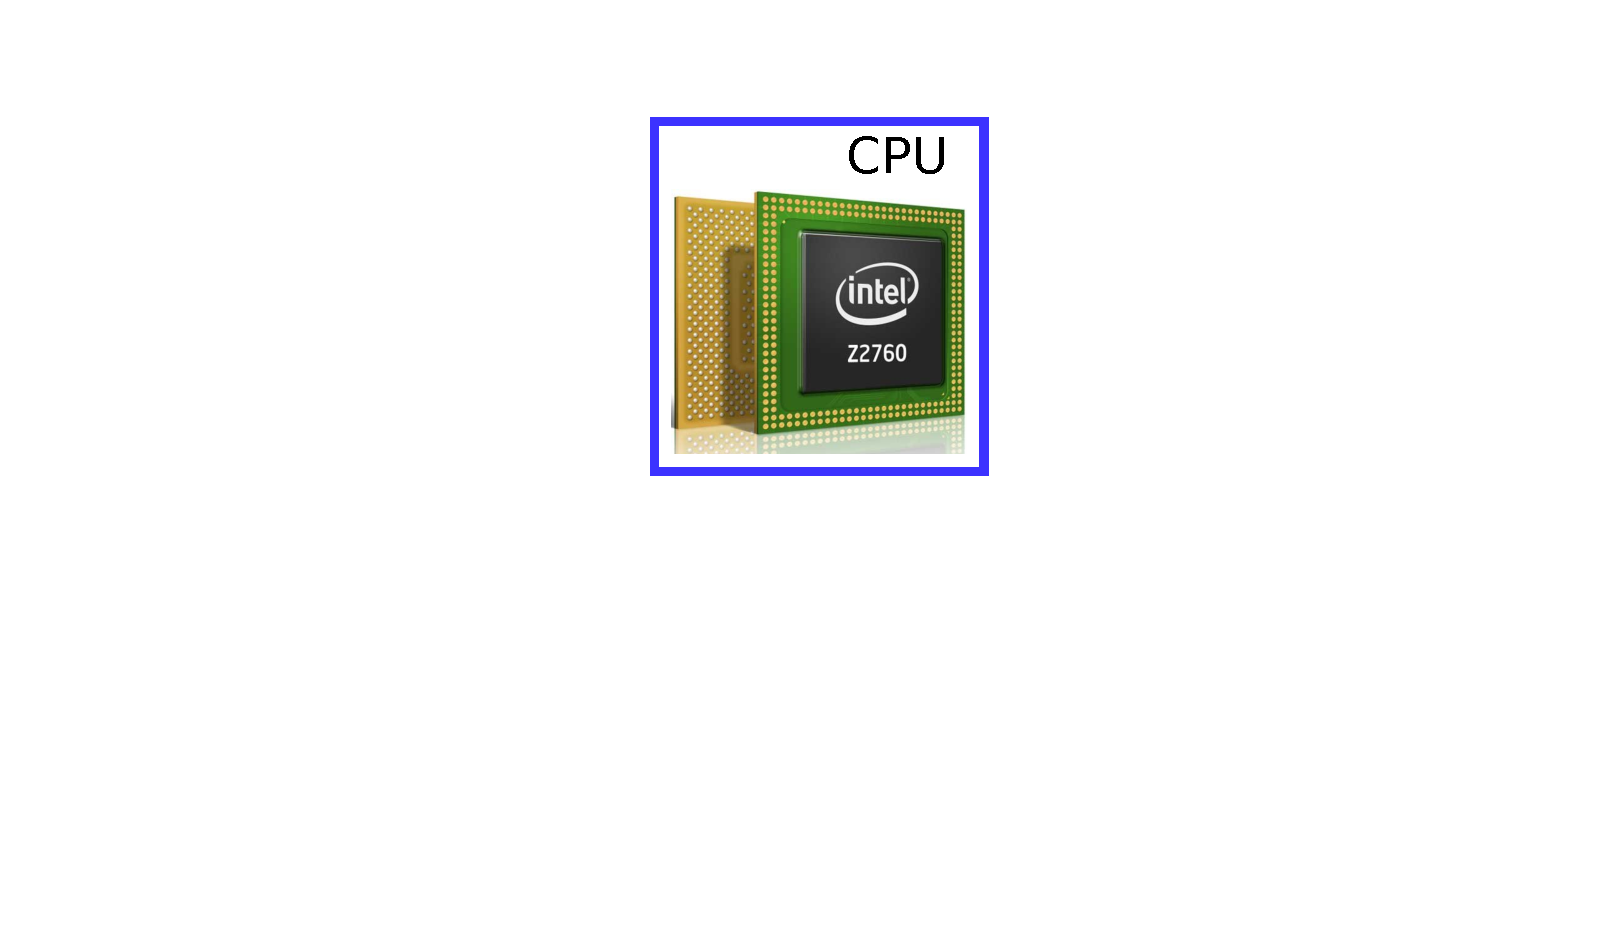
\includegraphics[width=\linewidth]{images/ordi_1.pdf}}
	%\only<2>{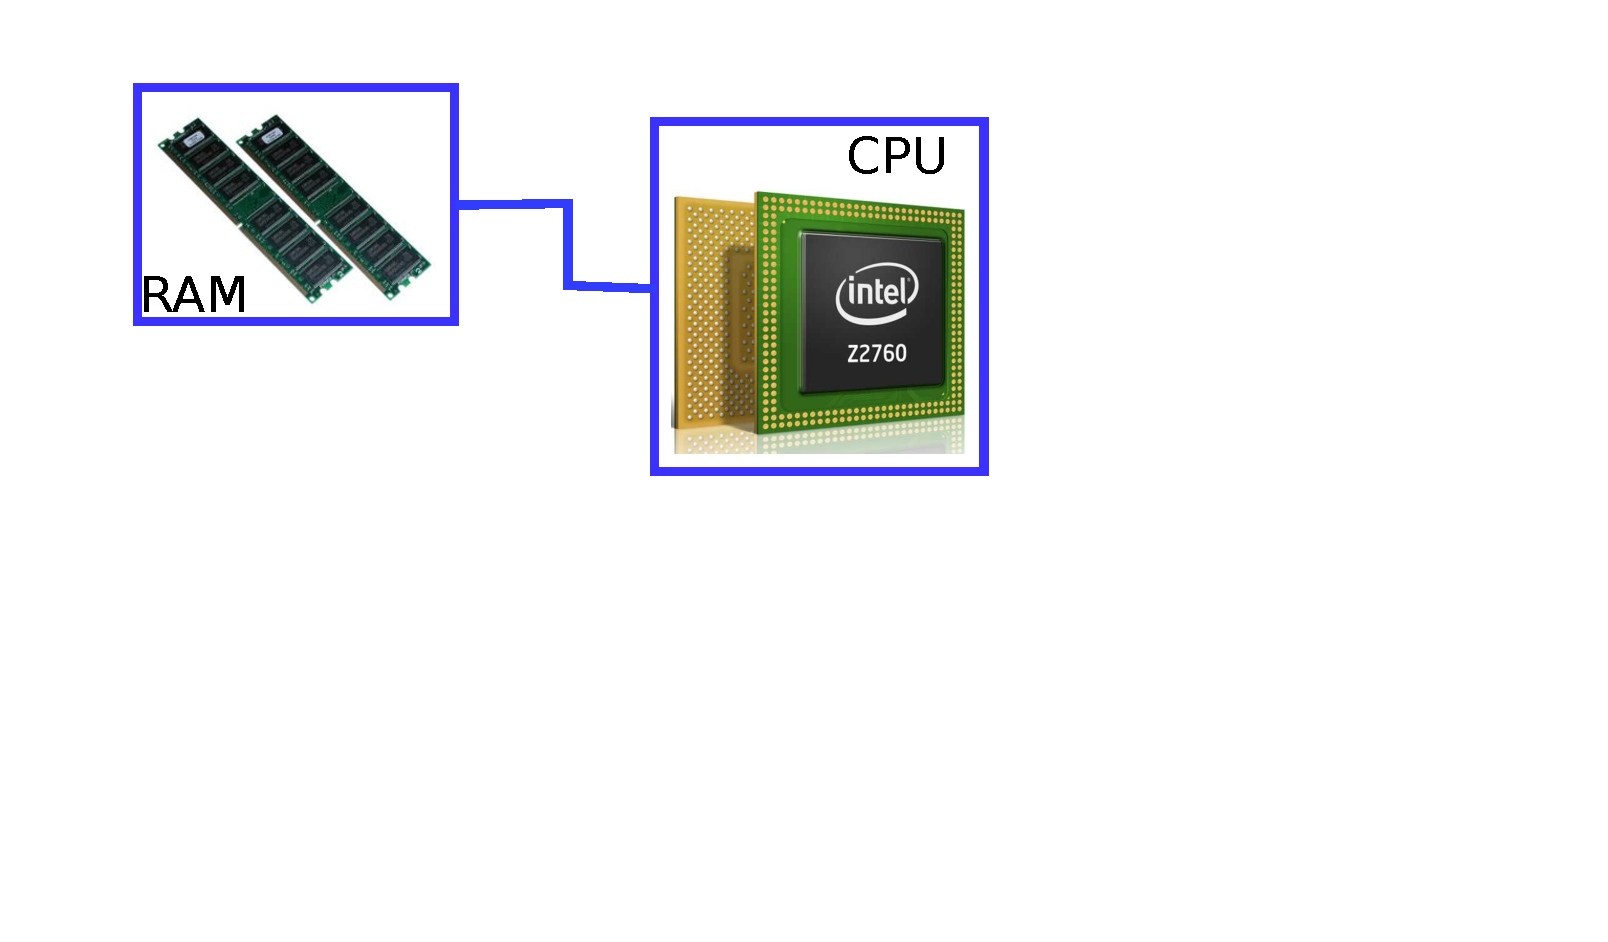
\includegraphics[width=\linewidth]{images/ordi_2.pdf}}
	%\only<3>{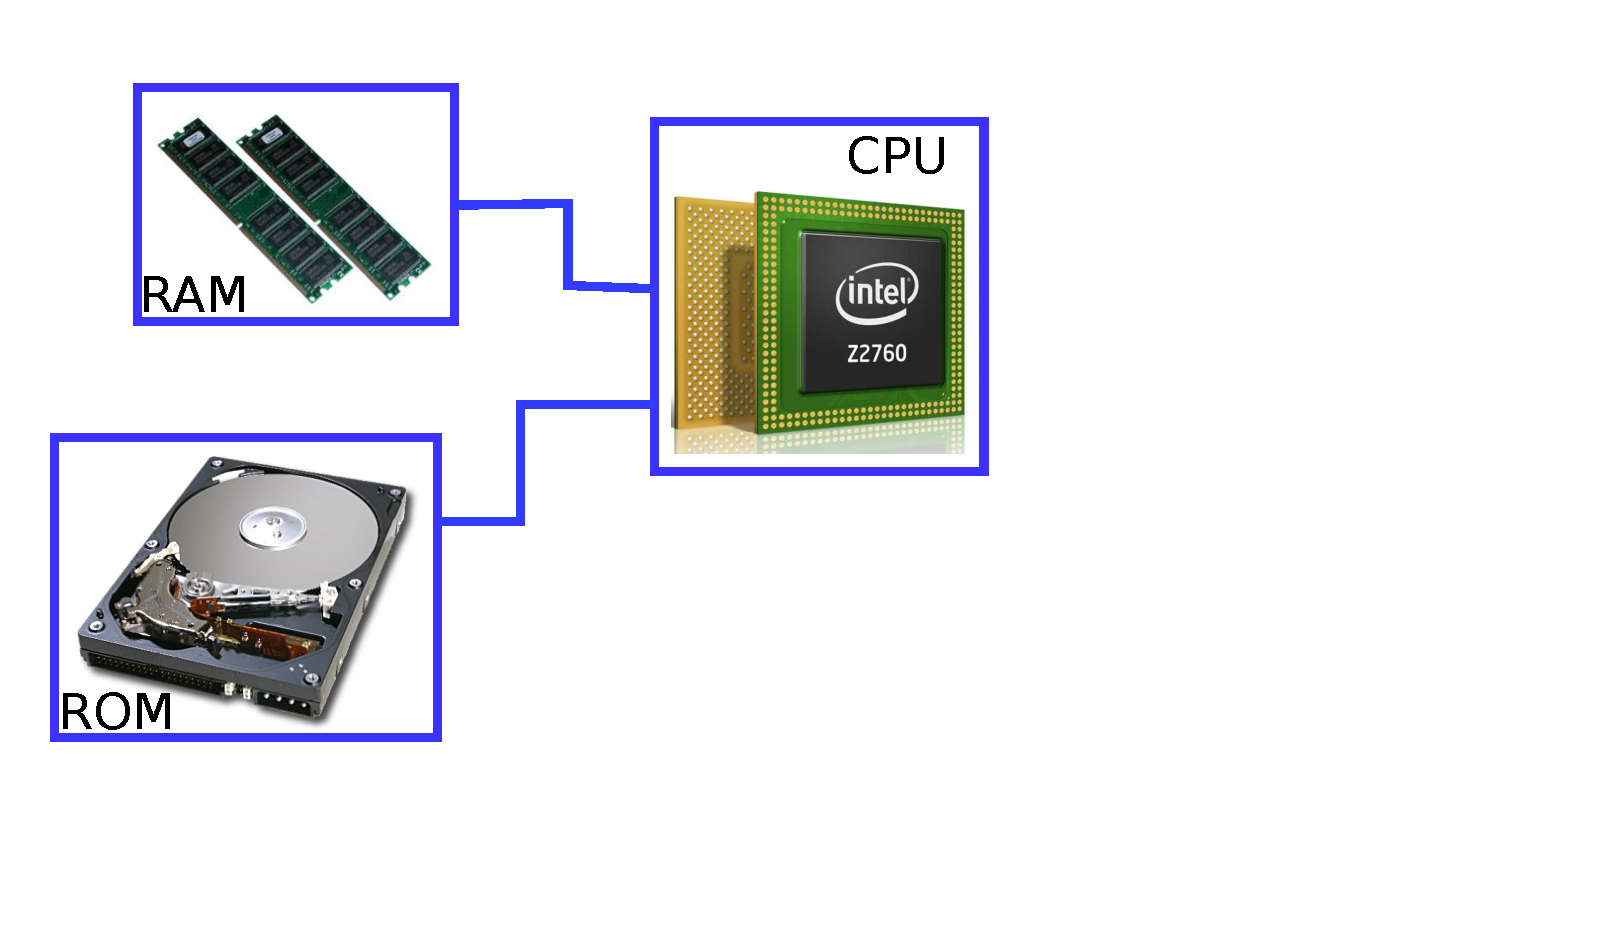
\includegraphics[width=\linewidth]{images/ordi_3.pdf}}
	%\only<4>{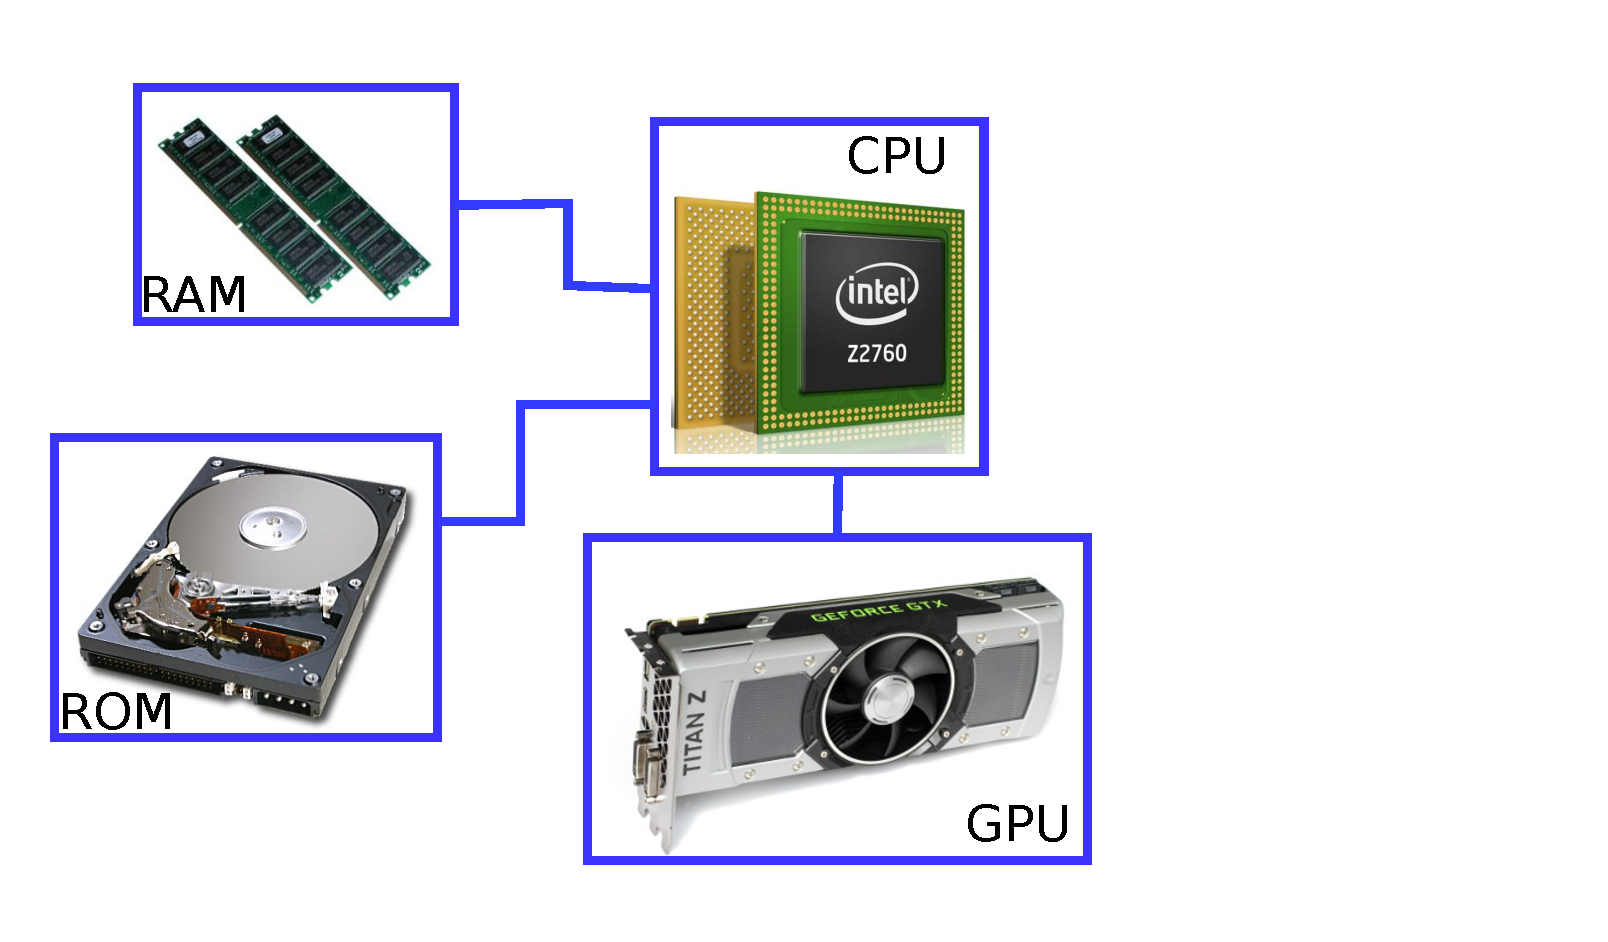
\includegraphics[width=\linewidth]{images/ordi_4.pdf}}
	%\only<5>{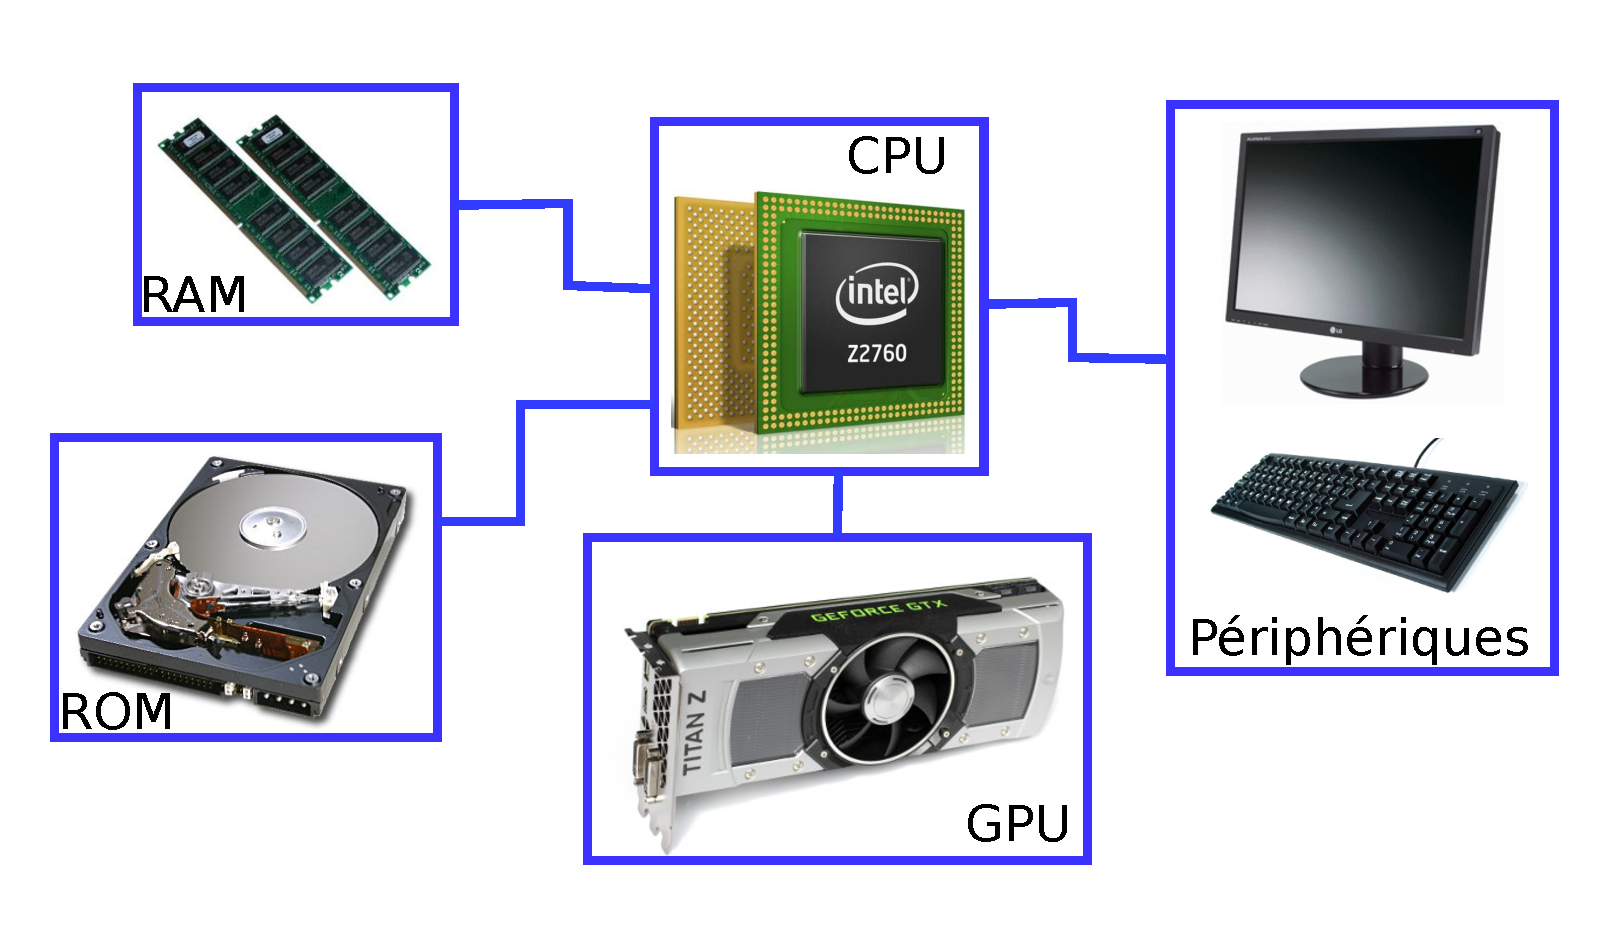
\includegraphics[width=\linewidth]{images/ordi_5.pdf}}
\end{frame}

\begin{frame}{Système d'exploitation}

  \begin{block}{OS (operating system)}
    Le système d'exploitation est le logiciel qui dirige les ressources de l'ordinateur. Il gère les périphériques et ordonne les tâches du processeur en fonction de leur priorité. Il s'occupe également de la mémoire vive et du stockage.
  \end{block}
  \vfill
  \begin{minipage}{0.25\linewidth}
	  
\includegraphics[width=\linewidth]{images/logo_windows10.jpg}
  \end{minipage}
  \hfill
  \begin{minipage}{0.25\linewidth}
	  
\includegraphics[width=\linewidth]{images/logo_ubuntu.png}
  \end{minipage}
  \hfill
  \begin{minipage}{0.25\linewidth}
	  
\includegraphics[width=\linewidth]{images/logo_osX.png}
  \end{minipage}
\end{frame}

\begin{frame}[fragile]{Langages de programmation}
  \begin{block}{Qu'est-ce qu'un langage de programmation ?}
  Un ensemble de symboles (syntaxe) et de règles d'écriture (grammaire) permettant de créer un programme.
  \end{block}
  \begin{minipage}{0.40\linewidth}
	\begin{itemize}[<+->]
		\item Langage machine (\textbf{assembleur})
		\item Langage exotique (Ook, \textbf{LOLCODE}\dots)
		\item Langage procédural (FORTRAN, \textbf{C}\dots)
		\item Langage objet (\textbf{C++}, Python, Java\dots)
		\item Langage fonctionnel (Lisp, \textbf{OCaml}\dots)
	\end{itemize}
  \end{minipage}
  \hfill
  \begin{minipage}{0.58\linewidth}
	\begin{overprint}
	\onslide<1>
	\begin{minted}{gas}
section .data
     helloMsg: db 'Hello world!',10
     helloSize: equ $-helloMsg
section .text
     global _start
_start:
     mov eax,4
     mov ebx,1
     mov ecx, helloMsg
     mov edx, helloSize
     int 80h
     mov eax,1
     mov ebx,0
     int 80h
	\end{minted}
	\onslide<2>
	\begin{minted}{basic}
HAI
CAN HAS STDIO?
BTW affiche le message
VISIBLE "Hello world!"
KTHXBYE
	\end{minted}
	\onslide<3>
	\begin{minted}{c}
#include<stdio.h>

int main()
{
    printf("Hello World!\n");
    return 0;
}
	\end{minted}
	\onslide<4>
	\begin{minted}{cpp}
#include <iostream>
using namespace std;

int main(){
  cout << "Hello world!" << endl;
  return 0;
}
	\end{minted}
	\onslide<5>
	\begin{minted}{ocaml}
print_endline "Hello world!"
	\end{minted}
	\end{overprint}
  \end{minipage}
\end{frame}

\begin{frame}{Compilé ou interprété ?}
	\begin{block}{Langages compilés}
		\begin{itemize}
		\item Le compilateur traduit à l'avance le code en instructions machines.
		\item Il transforme le code en un fichier exécutable (par exemple, \texttt{.exe} sous Windows).
		\item Exemples : C, C++, OCaml\dots
		\end{itemize}
	\end{block}
	\begin{block}{Langages interprétés}
		\begin{itemize}
		\item L'interpréteur traduit le code à la volée.
		\item Le code n'a pas besoin d'être transformé, mais l'interpèteur est indispensable.
		\item Exemples : Python, Ruby, PHP\dots
		\end{itemize}
	\end{block}
\end{frame}

\begin{frame}{Pourquoi programmer en C++}
    \begin{itemize}
        \item Un langage \textbf{complexe} : savoir programmer en C++ c'est savoir programmer dans tous les langages de la même famille (Java, C\#, Go, Rust\dots).
        \item Un langage \textbf{complet}, qui permet de travailler à haut niveau d'abstraction ou à bas niveau, proche de l'architecture de la machine.
        \item Un des langages \textbf{les plus utilisés}.
        \item Toujours en \textbf{évolution}/simplification.
    \end{itemize}
\end{frame}

\begin{frame}[fragile]{Python vs C++}
	\begin{itemize}
		\item Le Python est un langage interpreté, le C++ est un langage compilé.
		\item Le C++ sera en général plus rapide que le Python
		\item La délimitation des blocs se fait par des accolades \{\} (tabulation en Python)
		\item Chaque instruction se termine par un {\huge\textbf{;}}
		\item Les variables vivent dans le bloc où elles ont été créées.
	\end{itemize}
	\begin{minipage}{0.45\linewidth}
		\begin{minted}{python}
for id in range(10):
    a = id
print(a)
		\end{minted}
	\end{minipage}
	\hfill
	\begin{minipage}{0.45\linewidth}
		\begin{minted}{cpp}
for(int id=0; id<10; id++){
    a = id;
}
cout << a ;
		\end{minted}
	\end{minipage}
\end{frame}


\section{Premier programme}

\begin{frame}
  \frametitle{Structure des programmes}
  \centering
  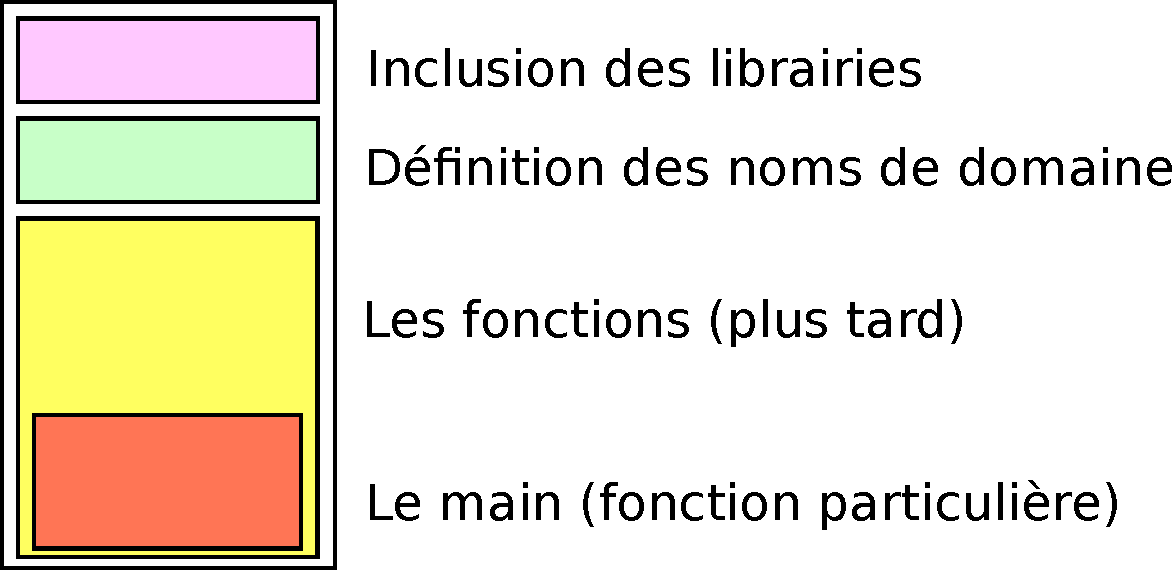
\includegraphics[width=\linewidth]{images/structure.pdf}
\end{frame}

\begin{frame}[fragile]
  \frametitle{Hello world}

  \begin{minted}{cpp}
// commentaire sur une ligne
#include <iostream>
/* commentaires par
 * bloc */

// utilisation du nom de domaine de la STL
using namespace std;

int main()
{
    cout << "Hello world!"; // écriture de "Hello world!"
    cout << endl; // passage à la ligne

    cout << "HelloWorld" << endl; // les deux en même temps

    return 0;
}
	\end{minted}
\end{frame}

\begin{frame}[fragile]
    \frametitle{Détails du programme : librairies}
    \begin{minted}{cpp}
        
#include <iostream>
        
    \end{minted}

    Appeler des libraires donne accès à des fonctions pré-existantes. \\
    C'est l'équivalent du \mintinline{python}{import ...} en Python.\\

    \texttt{\textbf{iostream}} fait partie de la Standard Template Library (STL).\\
    \texttt{\textbf{iostream}} permet de gérer les affichages à l'écran et de récupérer des entrées clavier.
\end{frame}


\begin{frame}[fragile]
    \frametitle{Détails du programme : nom de domaine}
    \begin{minted}{cpp}
using namespace std;
    \end{minted}

    En C++, les librairies peuvent avoir un nom de domaine (équivalent du nom de module en Python).

    Définir le nom de domaine permet de ne pas le répéter avec chaque fonction appelée, de façon similaire à \mintinline{python}{from ... import *} en Python.

\end{frame}

\begin{frame}[fragile]
    \frametitle{Détails du programme : la fonction main}
    \begin{minted}{cpp}
        
int main(){
    cout << "HelloWorld";
    cout << endl;
    cout << "HelloWorld" << endl;
    return 0;
}
        
    \end{minted}

    La fonction \texttt{\textbf{main}} est le point d'entrée du programme.\\
    Cette fonction est \textbf{obligatoire}.
\end{frame}


\begin{frame}[fragile]{Détails du programme : la fonction main}

    \begin{minted}{cpp}
        
int main(){ // type : int, nom : main, arguments : rien
        
    \end{minted}

    \texttt{\textbf{int}} est le type attendu du résultat de la fonction (ici un entier).\\
    \texttt{\textbf{main}} est le nom de la fonction.\\
    Le corps de la fonction (code) est compris entre des accolades.

    \begin{minted}{cpp}
        
    ...
    return 0; // valeur de retour lorsque tout s'est bien passé
}
        
    \end{minted}
    \texttt{\textbf{main}} renvoie un entier, ici $0$.
\end{frame}


\begin{frame}[fragile]{Détails du programme : le code}
    \begin{minted}{cpp}
        
    cout << "Hello world!";
    cout << endl;
    cout << "Hello world!" << endl;
        
    \end{minted}

    \texttt{\textbf{cout}} : mot-clé pour écrire à l'écran.\\
    \texttt{\textbf{"HelloWorld"}} est une chaîne de caractères.\\
    \texttt{\textbf{endl}} : mot-clé pour passer à la ligne.

    \begin{minted}{cpp}
        
    std::cout << "Hello world!"; // si on utilise pas le nom de domaine de la STL
    std::cout << std::endl;    // ie si pas de  using namespace std
    std::cout << "Hello world!" << std::endl;
        
    \end{minted}
\end{frame}

\begin{frame}{Quelques règles pour bien démarrer}
    \begin{itemize}
        \item Le code s'écrit \textbf{toujours} dans une fonction (le \texttt{main} pour l'instant).
        \item L'indentation (mise en forme) n'est pas nécessaire mais sera obligatoire dans le cours (lisibilité).
        \item Il y a une \textbf{unique} fonction \texttt{main} par programme.
    \end{itemize}
\end{frame}

\section{IDE, CMake, Imagine}

\begin{frame}
  \frametitle{IDE}

  \begin{block}{Integrated Development Environment}
      L'Environnement de Développement Intégré est un logiciel qui regroupe des fonctions pour aider le développeur, et ainsi gagner en productivité.
  \end{block}

  Il existe de nombreux IDE, spécialisés pour un ou plusieurs langages :
  \begin{itemize}
  \item \textbf{C++} : QTCreator, Eclipse, Microsoft Visual Studio, KDevelop, XCode\dots
  \item Python : Spyder, WingIDE, PyCharm...
  \item \dots
  \end{itemize}
\end{frame}

\begin{frame}{QtCreator}
    \textbf{QtCreator} est l'IDE que nous utiliserons dans ce cours.
    \begin{itemize}
        \item Multiplate-forme (Windows, Linux, OS X)
        \item Complet
        \item Relativement simple à utiliser
    \end{itemize}
\end{frame}

\begin{frame}{IDE et projets}
    Chaque IDE stocke les informations relative à un projet dans un format spécifique :
    \begin{itemize}
        \item L'emplacement des fichiers de code
        \item Les emplacements des librairies
    \end{itemize}
    Il est parfois fastidieux de construire un projet.

    Pour y remédier on utilise un \textbf{moteur de production}.

\end{frame}

\begin{frame}
  \frametitle{CMake}
  \textbf{CMake} est \textbf{moteur de production},  un logiciel pour tous les OS qui permet de générer les projets pour différents IDEs.

  \begin{block}{Utilisation}
	  \begin{itemize}
		  \item Interface utilisateur : Makefiles (Unix), Visual Studio (Windows), Xcode, Eclipse\dots
		  \item Directement dans l'IDE : QTCreator, KDevelop\dots
	  \end{itemize}
  \end{block}
\end{frame}

\begin{frame}[fragile]
  \frametitle{CMakeLists.txt}


Utilisation de fichiers de configuration :
\begin{minted}{cmake}  
CMAKE_MINIMUM_REQUIRED(VERSION 2.6)

#Inclusion des modules (ici Imagine++)
FILE(TO_CMAKE_PATH "$ENV{IMAGINEPP_ROOT}" d)
IF(NOT EXISTS "${d}")
  MESSAGE(FATAL_ERROR "Error: IMAGINEPP_ROOT=" "${d}")
ENDIF(NOT EXISTS "${d}")
SET(CMAKE_MODULE_PATH ${CMAKE_MODULE_PATH} "${d}/CMake")
FIND_PACKAGE(Imagine)

# Création d'un projet
PROJECT(TP1Supplement)
# Ajout d'un exécutable
add_executable(Tp1Supplement Tp1Supplement.cpp)
# Utilisation de Imagine++ (partie Graphics)
ImagineUseModules(Tp1Supplement Graphics)
\end{minted}
\end{frame}

\begin{frame}
	\frametitle{Déboguer avec l'IDE}
	Le débogueur est outil important de l'IDE par rapport au bloc-notes + ligne 
	de commande.

	Il permet d'exécuter le programme pas à pas et de détecter où se trouvent les erreurs dans le code.

	\begin{block}{QtCreator}
	dans l’onglet Projects, passer comme argument à CMake \textbf{\texttt{-DCMAKE\_BUILD\_TYPE=Debug}}
	\end{block}

	\begin{block}{MakeFiles}
	Passer \textbf{\texttt{CMAKE\_BUILD\_TYPE}} en \textbf{\texttt{Debug}}
	\end{block}

\end{frame}

\begin{frame}
  \frametitle{Librairie Imagine++}
  La librairie Imagine++ est une librairie graphique développée à l'ENPC.
  Elle contient :
  \begin{itemize}
      \item des fonctions pour l'affichage graphique (images, dessin\dots)
      \item le nécessaire pour l'agèbre linéaire de base (matrices, vecteurs\dots)
  \end{itemize}
\end{frame}

\end{document}
